{
{\sffamily I den udvidet løsning har vi valt, at se på den måde, vi vælger
ragioner ud på. Hvor vi i den naiveMethode valgte at se på ragionens bounding
box, vil vi i den udviden metode valje at se på mindre snit af ragionen, vi har
også valt at udvide måde vi bestemmer hvad en ragion er. En ragion var før,
ænden med eller ikke med i en snit. kommer den udvidelsen til at indeholde en
kateroesering af ragionerne, så en ragion kan have en vis katerogiering i
forhold til et snit.

Vi laver ikke om i vores feature detector.
}

\subsection{Udvidelse af ragioner plasering}
{
I denne udvidelse vil vi gerne indføre mere udføliger defination af
hvornår en ragion ligger i et snit. hvor vi før kun arbejdet med
ragionen som tagenteret inde i snittet, vil vi nu også gerne have
ragioner med som skæres i midden af snittet se figur
\ref{hus}.

\begin{figure}[h]
	\begin{center}
		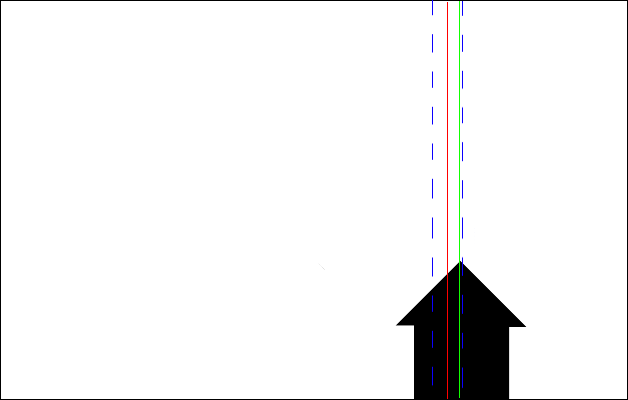
\includegraphics[scale=0.3,angle=0]{afsnit/vores_implementation/billeder/udvidet_loesning/husworks.png}
	\end{center}
	\caption[]{Et hus som bliver skåret over i midden af snittet}
	\label{hus}
\end{figure}

\subsubsection{Opdeling af ragion med et grid}
Måden vi deller ragionen op på, er hved hjælp af et gridt som vi
tilføjer vær baunding box, se figur \ref{grid}. Da vi ved hvilken farve
baunding boxens ragion er, tager vi alle de punkter i grittet som har
denne farve, og få der ved en bedre beskrivels af hvordan ragionen ser
ud. For at gøre algoritmen lidt hurtiger, er vores gridt punkter lavet
med 2 pixels mellemrum. XXX(dette rette vi nå vi pracis ved hvor stort
vores gridt er) XXX(har vi skravet at vi altid laver ragionerne
forskelige farver.)

\begin{figure}[h]
	\begin{center}
		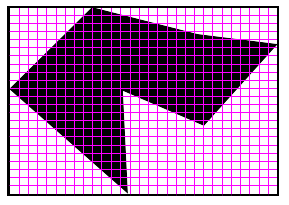
\includegraphics[scale=0.76,angle=0]{afsnit/vores_implementation/billeder/udvidet_loesning/udvidetloesninglayer.png}
	\end{center}
	\caption[]{Et grid over en ragion i baunding box}
	\label{grid}
\end{figure}

\subsubsection{Metode forklaring}
Vi har nu x antal punkter i en ragion og vi andtager at det er et af den
vertikale snit vi ser på. Så kan punkterne befinde sig oven på snittet,
til venstre eller til højre fra snittet. Alle punkterne har også en
afstand d til snittet og en afstand D til kanten af billedet. Med de 3
information kan vi sige en masse om ragionen, f.eks. skære snitte
ragionen i 2 lige store delle eller befinder næste helle figuren sig
lang væk fra snittet osv. Få at få nogle konkrate matematik ned, har vi
valt at se på disse 2 formler
\ref{MPunkt}, \ref{Fordeling}.

\begin{eqnarray} 
 MPunkt &=& \frac {\sum{D}}{x}\label{MPunkt}
\end{eqnarray}

\begin{eqnarray} 
 Fordeling &=& \frac{x_{venstre~side}-x_{højre~side}}{x}\label{Fordeling}
\end{eqnarray}

Formel \ref{MPunkt} finder et mid punktet af ragionen i forhold til
venstre side for vertikale snit og toppen ved højesuntale snit. se figur
\ref{midpunkt}

\begin{figure}[h]
	\begin{center}
		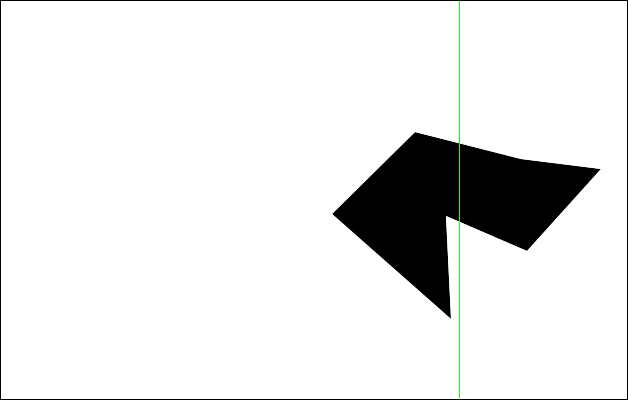
\includegraphics[scale=0.5,angle=0]{afsnit/vores_implementation/billeder/udvidet_loesning/centerOfmass.png}
	\end{center}
	\caption[]{ragion hvor masse midpunktet er tegnet in i forhold til venster side af billedet}
	\label{midpunkt}
\end{figure}

Vi sammen linier nu midpunktet med snittet og få en afstand, hvis denne
afstand er mindre en magien, så er ragione godtaget, se figur
\ref{cOMCutMargin}

\begin{figure}[h]
	\begin{center}
		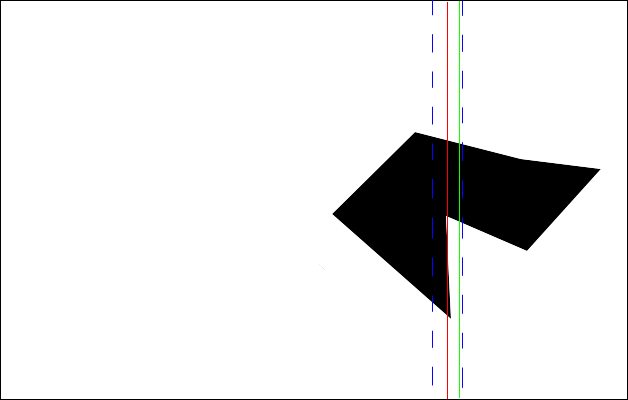
\includegraphics[scale=0.5,angle=0]{afsnit/vores_implementation/billeder/udvidet_loesning/cOMCutMargin.png}
	\end{center}
	\caption[]{ragion hvor masse midpunktet, snit og margin er teget ind, som man kan se ligger midpunktet inde for marginen}
	\label{cOMCutMargin}
\end{figure}

Nu skulle man tror at alting er godt men desværre kan vi kommer ud for
nogle figure som formel \ref{MPunkt} ikke tager højte for.

\begin{figure}[h]
	\begin{center}
		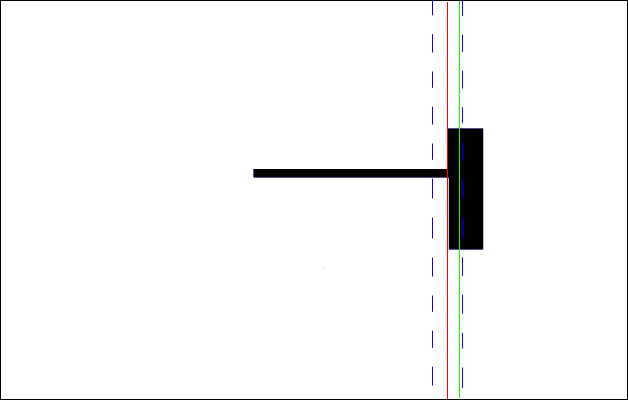
\includegraphics[scale=0.5,angle=0]{afsnit/vores_implementation/billeder/udvidet_loesning/dontWork.png}
	\end{center}
	\caption[]{Figur som overhold farmel \ref{MPunkt} men ikke \ref{Fordeling}}
	\label{dontwork}
\end{figure}

Som man kan se i figur \ref{Fordeling} er det fundene midpunkt inde for
marginen, men figur \ref{dontwork} har en lang stang som ænder med at
være lang væk fra snittet. Dette vil vi helt undgå da denne figur ikke
ligger i snittet. Men da de fleste pixels ligger på højre sider af
figuren kan vi, kan vi sotere denne figur væk ved at sammen line pixel
andtal på begge sider og se om den reletive pixeltal kommer under en vis
granse. Formel \ref{Fordeling} bruges til dette formål. Denne metode gør
også at vi få soteret de figure væk hvor snittet gå i gemmen side af
figuren, f.eks. et andsigt hvor snittet gå i gemmen kinden og ikke
næsen. se figur \ref{dontwork2}

\begin{figure}[h]
	\begin{center}
		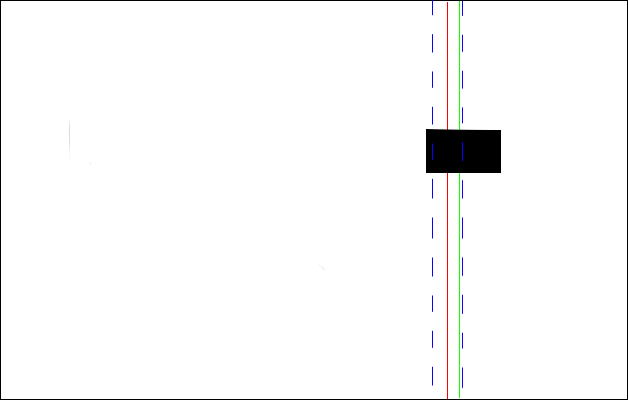
\includegraphics[scale=0.5,angle=0]{afsnit/vores_implementation/billeder/udvidet_loesning/dontwork2.png}
	\end{center}
	\caption[]{Figur som overhold farmel \ref{MPunkt} men ikke \ref{Fordeling}}
	\label{dontwork2}
\end{figure}

ud fra disse opsavatione, har vi indført de 3 kategoriera neden for.
kategori 1: Alle de ragioner som vi fand før med bounding box og $ |snit - MPunkt| \leq Q \wedge |Fordeling| \leq P_1$ \\
kategori 2: $|snit - MPunkt| \leq Q \wedge |Fordeling| \leq P_2 \wedge (snit - MPunkt)*fordeling \geq 0$ \\
kategori 3: Resten\\

Hvor Q er antal pixels mellem snittet og margien og $P_1$ og $P_2$ er procentvis forskel på de to sider.
Som man kan se vægter vi formlel \ref{MPunkt} højre en \ref{Fordeling}


\subsubsection*{brugbarhed}
\subsubsection*{Fordele vs ulember}

}

% vim: set tw=72 spell spelllang=da:


\subsection{Topografisk kort til omkostninger}
{
Et topografisk kort er et udtryk hentet fra geografi som er en
fremstilling af tærrenforskelle i et landskab. Traditionelle
topografiske kort bruger forskellige farver til at præsentere de
relative højder over havet. Denne metode kan bruges i andre sammenhænge,
f.eks. som vi vil gøre, ved at udskifte højde med en omkostning.
Eksempler på topografiske kort til klassificering af regioner i billeder
kan ses i figur \ref{topography_plus} og \ref{topography_times}.

Vi vil nu beskrive en metode hvorved regioner bliver tildelt en
omkostning. Denne omkostning beregnes ud fra regionens placering i
billedet på baggrund af et topografisk kort. Således vil regioner ikke
blive vurderet efter hvorvidt de ligger i det gyldne snit eller ej, men
efter \emph{hvor meget} de ligger i det gyldne snit.

\subsubsection*{Generering af topografisk kort}

Givet en afbildning af et maleri ved matricen $\mathbf{I}$ med dimensioner
$N \times{} M$, kan man opstille et topografisk kort $\mathbf{T}$ med dimensioner
$N \times{} M$.

Det topografiske kort generes ud fra to vektorer $\mathbf{X}^t =
\left(x_1, x_2, \cdots, x_n\right)$ og $\mathbf{Y} = \left(y_1, y_2,
\cdots, y_m\right)$ med dimensioner på henholdsvis $N \times 1$ og $1
\times M$.

Vi betragter vektoren $\mathbf{X}$ som liniestykket givet ved $AB$ i
figur \ref{topograph_line}. Længden af liniestykket betegnes ved $|AB|$.
Det følger af definitionen på $\mathbf{X}$ at $|AB| = n$. På liniestykket $AB$
er det gyldne snit placeret ved $G$ hvilket betegner indeks $\lfloor
n\varPhi \rfloor$ i $\mathbf{X}$. Et margin er angivet ved punkterne $(G
- \delta) = m$ og $(G + \delta) = m'$, hvor $\delta$ er størrelsen på
margin. Ligeledes betegner $m$ og $m'$ indeks $\lfloor n \varPhi \pm
\delta \rfloor$ i $\mathbf{X}$.  Endvidere har vi at $|Ap| = \lfloor
\frac{1}{2}|AB| \rfloor \leq |pB|$ og $|m'q| = \lfloor \frac{1}{2}|qB|
\rfloor \leq |qB|$. I figur \ref{topograph_line} er kun liniestykket
$pB$ segmenteret, men $Ap$ segmenteres symmetrisk.

Vi placerer nu et nyt punkt $x$ på $pB$. I det et-dimensionelle plan kan
længden $|Gx|$ bruges som mål for hvor tæt $x$ er på det gyldne snit.
Punktet $x$ har dog ingen udstrækning, hvorfor vi ikke blot kan bruge
længden i praksis. Vi betragter nu en region $R \in \mathbb{Z}^{+}$.
Regionen $R$ er en liniestykke i det et-dimensionelle plan. Vi kan da
udregne placeringen af $R$ i forhold til punktet $G$ ved at summere alle
afstandene fra punkterne $x$ i $R$ til $G$.  Dette medfører at lange
liniestykker bliver tildelt højere værdi end små. Vi udregner således
$\frac{\sum_{x \in R}{|Gx|}}{|R|} = |G(\frac{|R|}{2})|$, hvor $|R|$ er
længden, dvs. antallet af punkter i $R$. Dette svarer til at beregne
afstanden fra regionen midtpunkt til $G$. Dette er ikke ønskværdigt, da
vi kan have to regioner med forskellig længde, men med samme midtpunkt.
Hvis vi lader $R_{max}$ betegne den større region og $R_{min}$ være den
mindre, hvor $ \frac{|R_{max}|}{2} = \frac{|R_{min}|}{2}$, da må
$R_{max}$ nødvendigvis have et ekstrema tættere på $G$ end $R_{min}$.
Det er derfor ikke retfærdigt at give begge regioner den samme værdi.

Vi ønsker at belønne punkter der ligger i eller tæt ved det gyldne snit,
men give stor omkostning til punkter som ikke ligger i det gyldne snit.
Til dette bruges vektoren $\mathbf{X}$ angiver omkostningen for hvert
punkt på liniestykket $AB$. Da vi ønsker at belønne punkter i det gyldne
snit, tildels der ingen omkostning. Vi sætter derfor $\mathbf{X}_{|AG|}$
til $0$. Vi ønsker heller ikke at straffe regioner som ligger inden for
margin alt for meget. Vi sætter derfor $\mathbf{X}_{|Am|} =
\mathbf{X}_{|Am'|} = 1$, hvilket angiver omkostningen for at ligge på
margin. Værdierne mellem det gyldne snit og margin interpoleres således
at vi har en lineær overgang. Passende værdier vælges til
$\mathbf{X}_{|Ap|}$, $\mathbf{X}_{|Aq|}$ og $\mathbf{X}_{0} =
\mathbf{X}_{|AB|}$, hvor der ligeledes interpoleres mellem punkterne.
Liniestykket bliver således delt ind i nogle sektorer, som har en vis
omkostning alt efter hvor tæt man ligger på snittet. Derved kan vi undgå
ovenstående eksempel, hvor to regioner gives samme omkostning på trods
af at de har forskellig størrelse.

\begin{figure}[!h]
    \centering
    \begin{picture}(240,30)
        \put(0, 10){$A$}
        \put(3, -5){\line(0, 1){10}}

        \put(116, 10){$p$}
        \put(118, -5){\line(0, 1){10}}

        \put(131, 10){$m$}
        \put(134, -4){\line(0, 1){8}}

        \put(144, 10){$G$}
        \put(147, -4){\line(0, 1){8}}

        \put(157, 10){$m'$}
        \put(160, -4){\line(0, 1){8}}

        \put(195, 10){$q$}
        \put(198, -4){\line(0, 1){8}}

        \put(233, 10){$B$}
        \put(236, -5){\line(0, 1){10}}

        \put(182, 10){$x$}
        \put(185, 0){\circle*{3}}

        \put(3, 0){\line(1, 0){233}}
    \end{picture}
    \caption[]{Liniestykke}
    \label{topograph_line}
\end{figure}

\paragraph{Omkostningsfunktionen}
Vi vil nu overføre det ovenstående til to dimensioner. Det er trivielt
at opdele vektoren $\mathbf{Y}$ på samme måde som $\mathbf{X}$. Vi
ønsker at beregne en omkostning ud fra værdierne i vektorerne ved en
given koordinat. Vi definerer en funktion $t :
\mathbb{Z}^{+} \times \mathbb{Z}^{+} \rightarrow \mathbb{R}_{0}$ ved
\begin{equation}
    t(x, y) = \mathbf{X}_x + \mathbf{Y}_y
    \label{topo_plus}
\end{equation}
Det topografiske kort, som angivet ved funktionen \ref{topo_plus}, kan
ses i figur \ref{topography_plus}. Omkostninger er illustreret ved
mængden af hvid farve. Kortet viser at der ikke er nogen omkostning i
punktet $(G, G)$. Endvidere ses det at omkostningen er høj for punkter
ved hjørnerne og ved kanterne generelt. Dog kan man ret tydeligt se
grænserne mellem regionerne, da der interpoleres lineært.

Vi kan lave en mere flydende overgang mellem regionerne ved at definere
en ny funktion $u : \mathbb{Z}^{+} \times \mathbb{Z}^{+} \rightarrow
\mathbb{R}_{0}$ ved
\begin{equation}
    u(x, y) = \mathbf{X}_x\mathbf{Y}_y
    \label{topo_multiply}
\end{equation}
hvor vi multiplicerer omkostningerne i stedet for at addere dem. Det
resulterende topografiske kort ses i figur \ref{topography_times}. Da vi
nu bruger multiplikation vil vi gange med $0$ i det gyldne snit, hvorfor
dette er meget mere fremstående. Det skal dog nævnes at det ikke er helt
hensigtsmæssigt at omkostningen er meget lav ude ved ekstremerne.
Funktionen $u$ mangler altså den gode egenskab fra $t$ hvor ekstremerne
har store omkostninger.  Vi ser dog en eksponentiel stigning i
omkostningerne når vi bevæger os længere væk fra det gyldne snit.
Optimalt ville man have den samme omkostning ved ekstremerne som i $t$,
men med den eksponentielle stigning som i $u$.

Vi kan nu beregne omkostningen for en interessant region. Givet en
mængde $R \in \{\mathbb{Z}^{+}\times\mathbb{Z}^{+}\}$, som angiver
punkterne i en region, kan man finde omkostningen $C$ ved
\begin{equation}
    C(R) = \sum_{(x, y) \in R}{\frac{\tau(x, y)}{|R|}}
\end{equation}
hvor $\tau$ er en funktion fra $\mathbb{Z}^{+}\times\mathbb{Z}^{+}$ ind
i $\mathbb{R}_0$ som beregner omkostningen for et punkt fra et
topografisk kort. Vi har foreslået funktionerne $t$ og $u$. Jo lavere
omkostning en region har, jo bedre er den placeret i forhold til det
gyldne snit. I praksis er det oplagt at approksimere regionens
størrelse ved at bruge et gitter, ligesom i det foregående afsnit.


\begin{figure}[h]
    \setlength\fboxsep{0pt}
    \setlength\fboxrule{0.5pt}
    \begin{center}
        \fbox{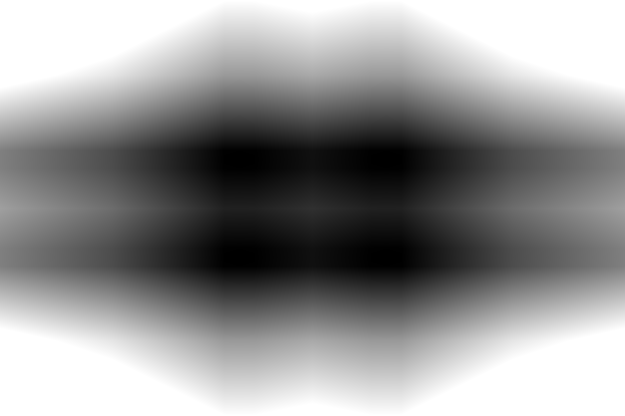
\includegraphics[width=0.8\textwidth]{afsnit/vores_implementation/billeder/udvidet_loesning/topographic_plus.png}}
    \end{center}
    \caption[]{Topografisk kort angivet ved funktionen $t(x, y) =
    \mathbf{X}_x + \mathbf{Y}_y$. Mængden af hvid farve reflekterer
    omkostningen. Helt hvid er dyrest, mens sort er billigst.}
    \label{topography_plus}
\end{figure}

\begin{figure}[h]
    \setlength\fboxsep{0pt}
    \setlength\fboxrule{0.5pt}
    \begin{center}
        \fbox{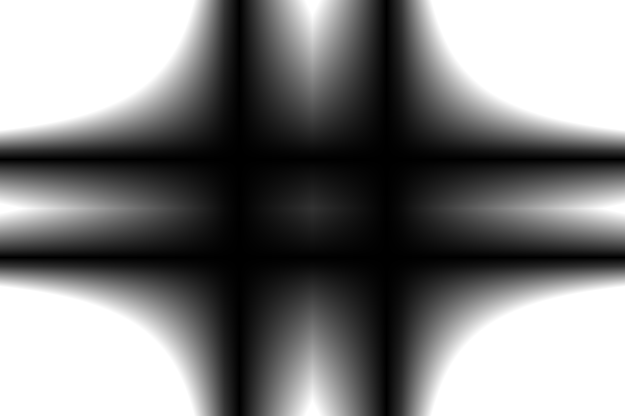
\includegraphics[width=0.8\textwidth]{afsnit/vores_implementation/billeder/udvidet_loesning/topographic_times.png}}
    \end{center}
    \caption[]{Topografisk kort angivet ved funktionen $u(x, y) =
    \mathbf{X}_x\mathbf{Y}_y$. Vi har igen, at hvid farve reflekterer
    omkostningen. Bemærk hvordan det gyldne snit er fremhævet.}
    \label{topography_times}
\end{figure}

\subsubsection*{Fastsættelse af omkostninger}
Det er let at se, at udformningen af det topografiske kort ikke blot
afhænger af funktionen $\tau$, men mere af de værdier man tildeler
omkostningsvektorerne. Værdierne, som er tildelt i det ovenstående, er
valgt arbitrært efter det bedste grafiske resultat. Vi har tidligere
nævnt, at værdierne interpoleres lineært. Hvis man adderer værdierne er
denne metode ikke helt hensigtsmæssig. Det er dog oplagt at gøre brug af
normalfordelingen til at fastsætte omkostninger. Dette skal dog ses med
omvendt fortegn, hvilket betyder, at vi nu tildeler regioner points. Man
kan altså basere antallet af points for et punkt i det et-dimensionelle
plan, ved at bruge en normalfordeling $N(\mu, \sigma)$ med middelværdi
$n\varPhi$ og en passende varians til margin. Umiddelbart ville man
sætte standardafvigelsen til $\delta$, vores margin, hvilket giver os en
varians på $\sigma^{2} = \delta^{2}$. Dette giver os en meget spids
normalfordeling, hvor punkter bliver tildelt mange points for at ligge
inden for margin, men hurtigt aftager når man bevæger sig længere væk.

%\subsubsection*{Fordele og ulemper}
%Brug af omkostninger ved topografiske kort har den umiddelbare fordel at
%kunne tildele regioner en værdi og derved være mere nuanceret i
%bedømmelsen af regioner. Metoden afhænger dog af fornuftige værdier i
%omkostningsvektorerne.

}

% vim: set tw=72 spell spelllang=da:


\subsection{Beslutning}
Hvilken udvidelse har vi valgt at implementere?

}

% vim: set tw=72 spell spelllang=da:

